\documentclass[12pt]{article}

%% Language and font encodings
%% doesn't work on my laptop
%\usepackage[english]{babel}
\usepackage[utf8x]{inputenc}
%\usepackage[T1]{fontenc}
\usepackage{amsmath}
\usepackage{pdfpages}

%% Sets page size and margins
\usepackage[letterpaper,top=1in,bottom=1in,left=1in,right=1in,marginparwidth=1in]{geometry}

%% Useful packages
\usepackage{amsmath}
\usepackage{graphicx}
%\usepackage[colorinlistoftodos]{todonotes}
\usepackage[colorlinks=true, allcolors=blue]{hyperref}

\usepackage[round]{natbib}
\setlength{\bibsep}{0.0pt} % compactify?

\usepackage[normalem]{ulem}
\usepackage{hyperref}
\usepackage{fancyhdr}
\pagestyle{fancy}
\fancyhead{} % clear all header fields
\renewcommand{\headrulewidth}{0pt} % no line in header area
\fancyfoot{} % clear all footer fields
%\fancyfoot[LE,RO]{\thepage}           % page number in "outer" position of footer line
\fancyfoot[RE,LO]{\footnotesize{T. Jaffe -- Project Description -- 3712 for NSF 18-575}} % other info in "inner" position of footer line

\newcommand{\planck}{\textit{Planck}}
\newcommand{\wmap}{\textit{WMAP}}
\newcommand{\imagineC}{IMAGINE Consortium}
\newcommand{\imagine}{\textsl{IMAGINE}}
\newcommand{\imagineSW}{\textsl{IMAGINE}}
\newcommand{\hammurabi}{\textsl{hammurabi}}
\newcommand{\hammurabix}{\textsl{hammurabi\,X}}
\newcommand*\mnras{MNRAS}
\newcommand*\apj{ApJ}
\newcommand*\apjl{ApJL}
\newcommand*\aap{A\&A}

\newcommand{\cpuh}{CPU\,h}
\newcommand{\GHz}{{\rm GHz}}  %Gigahertz


\definecolor{red}{rgb}{1, 0.0, 0}
\newcommand{\todo}[1]{\textcolor{red}{#1}}


\title{\vspace{-2cm}IMAGINE magnetic fields and the CMB}
\author{T. R.  Jaffe}

\begin{document}

\pagenumbering{gobble}


\section*{Intellectual Merit}


\subsubsection*{Context:  the Galactic magnetic field}\label{sec:gmfs}

Though the Galactic magnetic field (GMF) is important for many astrophysical processes in the interstellar medium (ISM) and for the dynamics of the Galaxy as a whole, its strength, coherence, and large-scale morphology are not yet understood.  A variety of models have been proposed in the literature, generally adapted to match only one or two observables and often incompatible with others. Figure \ref{fig:gmfs} shows the three GMF models compared in \citet{pipXLII} (hereafter, PIPXLII): on the {\it left} is from \citet{sun08} (Sun08); in the {\it middle} is from \citet{jansson12b} (JF12); on the {\it right} is \citet{Jaffe:2013} (Jaffe13). While morphologically quite different, each is consistent, depending on the underlying assumptions, with the most common probes of the GMF:  the diffuse synchrotron emission and Faraday rotation measures (RMs). Even though the models have been fit to the same data, the different numbers of parameters varied and the different assumptions that were made prevent a simple comparison of $\chi^2$ from determining which model is the most informative.  The first goal of this proposal is to quantitatively compare these models and from there to improve them so that we can then exploit them to understand both the propagation of cosmic rays (CRs) in the Galaxy and the impact of the Galactic emission on cosmic microwave background (CMB) observations.

The correct way to compare such models quantitatively is with the so-called Bayesian evidence, the statistical approach that takes into account the size of the parameter space as well as any prior information. This has not been done before. More importantly, none of the models have been correctly optimized on the full sky. The Sun08 model was only roughly fit 'by eye'. The JF12 model was optimized with a Markov Chain Monte Carlo (MCMC) method, but the ``galactic variance'' (the expected variation among galaxy realizations of a particular model, of which our own Galaxy is only one example) was not included explicitly, only approximately. The Jaffe13 model was optimized with MCMC and included the galactic variance, but only in the Galactic plane. Each analysis chose a different, and feasible, subset of the problem to tackle. But the conclusions remain highly uncertain. The JF12 model claimed to detect an x-shaped halo field around the Galaxy, which would have interesting implications for theories of Galactic outflow.  But as demonstrated in PIPXLII, there were significant shortcomings in the data they chose to use in addition to the variance issue. The Sun08 model required a significant enhancement of the local cosmic ray density, a value that is much higher than suggested by any results from direct measurements or indirect $\gamma$-ray observations. This density uncertainty translates directly into an uncertainty in the degree of ordering in the magnetic field, a crucial property for understanding the turbulence and dynamics in the ISM.  The Jaffe13 model includes the first measurement \citep{jaffe10} of the anisotropic random (aka ``striated'') component of the field in the plane, but that analysis did not probe the 3D properties due to the computationally challenging nature of the problem and the resources available. 

The first step is to provide the community with a quantitative Bayesian comparison of each of these models from the literature using the \imagineSW\ framework\footnote{\url{https://www.astro.ru.nl/imagine/}} \citep{imagineWP}.  A white paper on the project as a whole \citep{imagineWP} describes not only the infrastructure but also the many scientific domains it includes, among them the analysis of MHD simulations and the study of turbulent Galactic foregrounds.  Furthermore, forthcoming C-Band All Sky Survey (CBASS; see \citealt{cbass}) data will improve the synchrotron modeling by providing a crucial frequency in a spectral gap that  is currently limiting the synchrotron modeling  (as described in detail in PIPXLII).  The next step in understanding the GMF is then to be able to quantify which individual features of these models (e.g., x-shaped halo field; field reversals; a local CR enhancement; etc.) can be unambiguously measured and to construct a parametrization (or more likely a set of parametrizations) that include these features in the most generic and physically realistic way. This is the program we propose for the first part of the project. 


\begin{figure*}
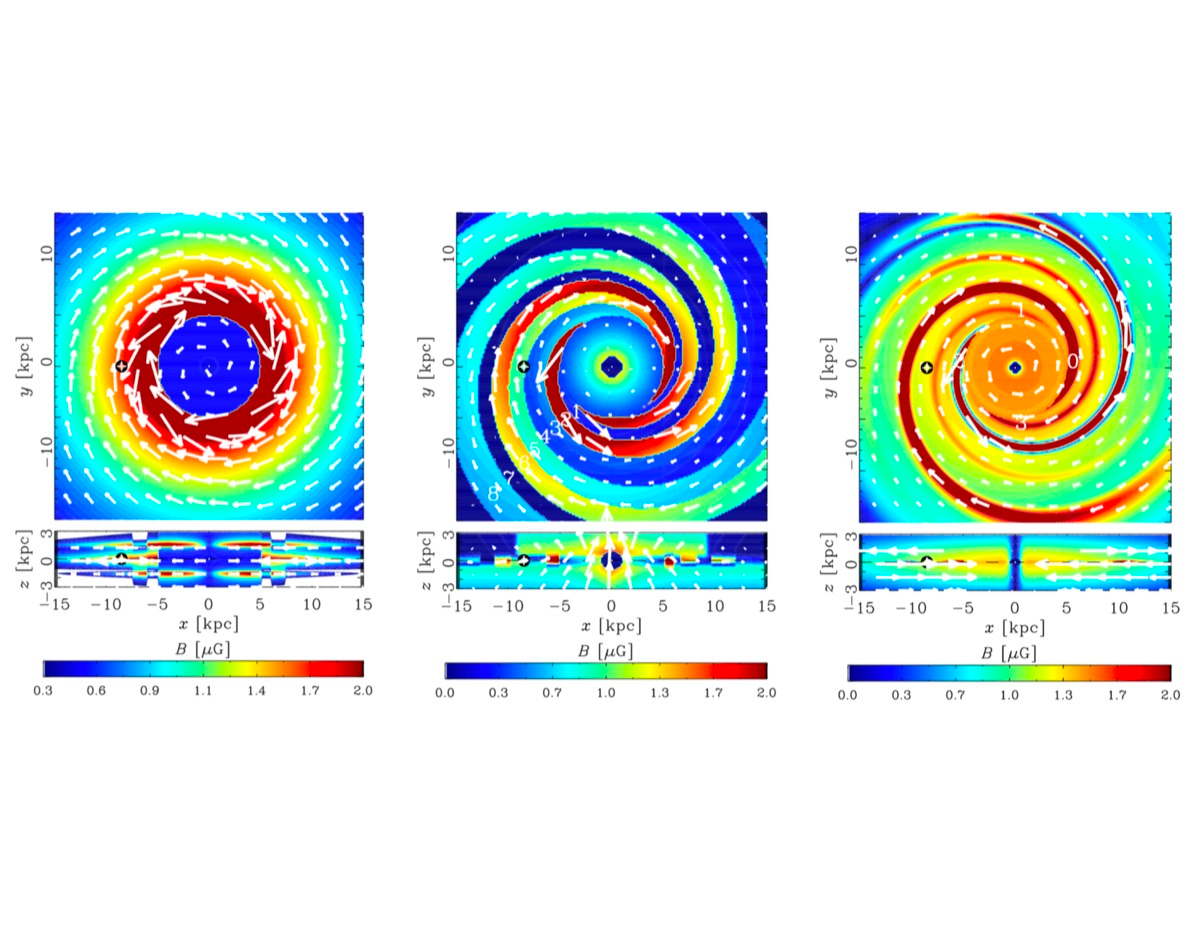
\includegraphics[width=\textwidth]{views_lowres.pdf}
\caption{Three GMF models analyzed in \citet{pipXLII}, from {\bf left}
    to {\bf right}: Sun08, JF12, and Jaffe13 (see text). In 
color is the strength of the coherent magnetic component, while the white arrows show its direction. The top panel of each shows a cut through the Galactic plane at $z=0$ with the Sun position marked by the black plus, while the bottom panel of each shows a vertical cut intersecting the Sun and the Galactic center.} 
\label{fig:gmfs}
\end{figure*} 

\subsubsection*{Context:  sub-mm observations and the CMB}

The \planck\ mission's primary goal was to map the temperature fluctuations in the CMB.  Polarization was an addition that turned out to be far more interesting than anticipated, both for cosmologists and Galactic astrophysicists. Though the Galactic emission is a nuisance to cosmologists, it is also a rich source of information about various astrophysical and astroparticle properties of the ISM. At low frequencies, the \planck\ bands are dominated by the synchrotron emission from relativistic cosmic-ray electrons accelerated in the Galactic magnetic field. In the submm bands, they are dominated by thermal emission from rotating dust grains that tend to align themselves with the GMF.  Full-sky maps of the polarization information are shown in Fig.\,\ref{fig:planck}.   Because the synchrotron emission comes from a much more diffuse population of relativistic cosmic rays while the dust emission comes from dust distributed in a very thin and clumpy Galactic disk, they provide complementary information about magnetic fields in different phases of the ISM.  Fully exploiting their complementarity is the second goal of this proposal.  

%Radio astronomy has long studied the longer wavelength synchrotron emission at a variety of frequencies, but the \planck\ and \wmap\ data provide the only full-sky sky maps of this component at frequencies high enough to avoid the Faraday depolarization effects that erase the information beyond a few hundred parsecs. The polarized dust emission in the submm bands is equally unique and has provided an unprecedented view of the small-scale turbulent structures in the colder regions of the magnetized ISM. 

%On large angular scales, PIPXLII showed how the combination of polarized synchrotron and dust emission could be used to constrain the large scale GMF. But that paper also demonstrated the difficulty interpreting the results of different model fits as well as the various challenges in the analysis that lead to different assumptions made by each team.  The \imagineSW\ framework \citep{imagineWP} will allow us to perform a systematic analysis of the models in PIPXLII and to compare them in a quantitative rather than qualitative way. 

On small angular scales, \citet{pipLIV}, for example, and citations therein, describe some of the properties of the dust in the turbulent ISM that we are only beginning to learn about. 
%Radio astronomy has been studying the turbulent ISM with synchrotron, but not at higher frequencies where Faraday effects are negligible.  
Though much of the effort regarding CMB foregrounds has focused recently on dust emission, the synchrotron emission cannot be neglected, and the turbulence in both dust and synchrotron emission need to be understood together in order to fully characterize the CMB foregrounds.  Our collaborator F. Boulanger is developing new statistical analysis methods and applying them to MHD simulations that focus on the cold dusty ISM.  Another collaborator A. Shukurov has cosmic-ray driven MHD turbulence simulations. We will combine these simulations with our \hammurabi\ observable generator \citep{waelkens:2009} to produce more realistic full-sky maps of ISM turbulence in the microwave and submm bands than ever done before. An example simulation is shown in Fig.~\ref{fig:mhd}. To these simulations, we can apply statistical tools already applied to the \planck\ data in order to determine how to use the information in the data to constrain the MHD theory. 


\begin{figure*}[]
%$\begin{array}{llrr}
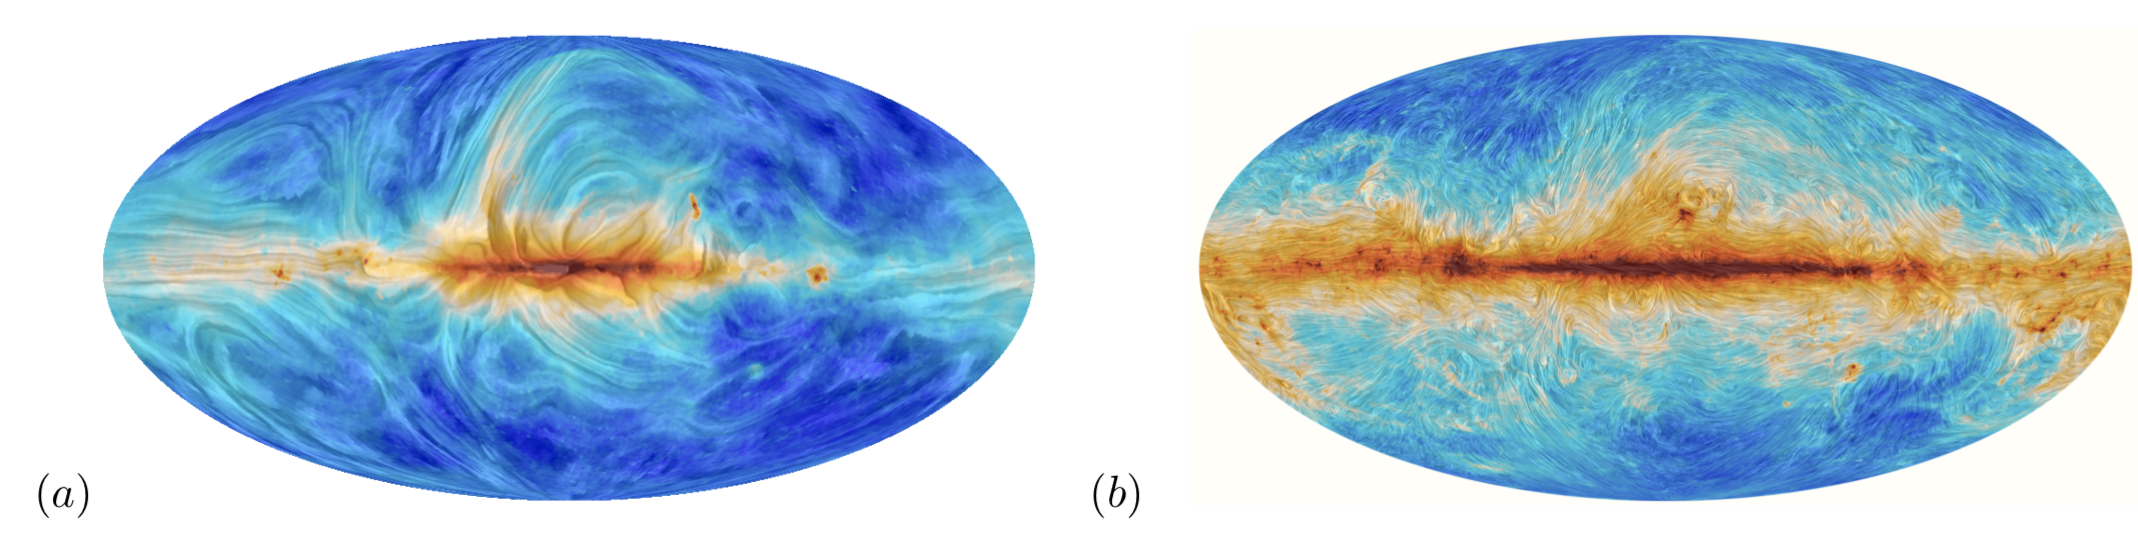
\includegraphics[width=\columnwidth]{maps_lowres.png}
%(a)\includegraphics[width=0.45\columnwidth]{2015_30GHz_B-field.pdf}&(b)&\includegraphics[width=0.45\columnwidth]{2015_353GHz_B-field.pdf}
%\end{array}$
 \caption{Synchrotron emission at $30\,\GHz$ ({\bf left}) and dust emission at $353\,\GHz$ ({\bf right}).
The color indicates the total intensity, while the texture applied shows the inferred plane-of-sky magnetic field direction, i.e.\ the polarization direction rotated by $90
\deg$.
See \citet{planck15_I}. Image credit: ESA and the Planck Collaboration.}
%% Note on image reproduction:  http://www.esa.int/spaceinimages/ESA_Multimedia/Copyright_Notice_Images
\label{fig:planck}
\end{figure*}


The next major breakthrough in cosmology with the CMB is expected to come from the search for the signal of primordial gravitational waves. In CMB terminology, we are looking for the so-called B-mode polarization signal, i.e., a pattern in the anisotropies that is divergence-free and arises only from gravitational waves, unlike the curl-free E-modes generated by a number of later processes. Inflation theories predict a B-mode polarization signal at an unknown level that, if measured, would constrain the space of allowed theories. Numerous CMB experiments are underway or planned to search for these signals. 
%\planck\ was able to place upper limits on the tensor-to-scalar ratio that controls the amplitude of the signal. 
The difficulty for all future missions is the fact that the polarized sky is largely dominated by emission from our own Milky Way galaxy, and that its signal mixes into both the E- and B-modes of the CMB anisotropies. The numerous \planck\ results produced by F. Boulanger's group (\citealt{pipLIV} and references therein)  have demonstrated how the turbulent dust foreground affects both the ratio of E- to B-modes as well as the TE correlation.  In order to detect the inflation signal, we need to understand these effects in the context of the MHD turbulence, how they affect both dust and synchrotron emission, and how they feed into the potential instrument systematics. The latter problem in particular was a central topic at a recent workshop on how to define the next-generation CMB project (``Designing Future CMB Experiments'', March 2018, funded by the Keck Institute for Space Studies, report forthcoming). 

%The processes that control both the propagation of cosmic rays and the formation of dusty structures in the ISM are not well understood. The largely separate field of MHD theory is also producing increasingly powerful and high resolution 3D simulations with wide dynamic ranges and more realistic conditions. What has been missing until recently are tools to connect these active fields of theory and observation. Recent studies such as \citet{Burkhart:2012} have begun to make such connections in the radio. But this has not yet been done for dust emission or for synchrotron emission in the microwave bands over large angular scales. 

%The \imagineSW\ framework now gives us the tools to put all these
%pieces together. We have an ambitious, long-term project, and this
%ADAP proposal would be a first step. 


\begin{figure}[t]\centering
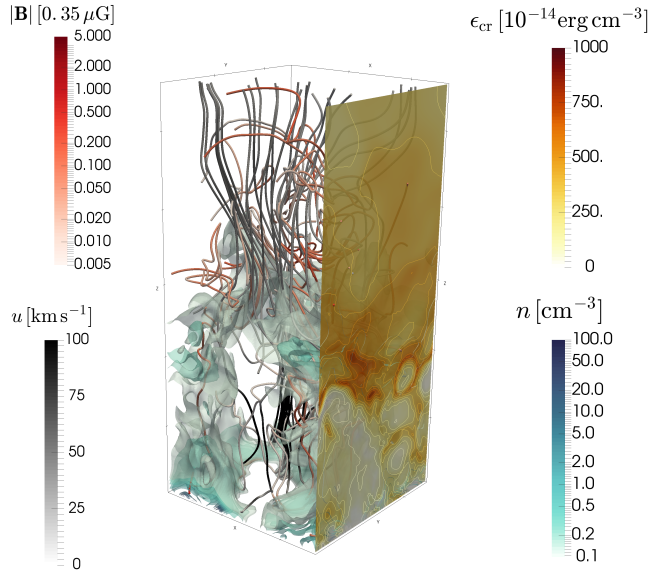
\includegraphics[width=0.7\columnwidth]{CR_box_low-res.png}
\caption{ An example of an MHD simulation from A. Shukurov and G. Sarson. Isosurfaces of gas density $n$ ({\bf blue}), magnetic field $\vec{B}$ lines ({\bf red}), gas 
velocity $\vec{u}$ streamlines ({\bf black}) and cosmic ray energy density $\epsilon_{\mathrm{cr}}$ ({\bf contours} 
on the right-hand face), in MHD simulations of the supernova-driven, multi-phase ISM 
that extend the simulations of 
\citet{Gent:2013b} 
by the inclusion 
of cosmic rays. Holes in the density distributions are supernova remnants. Note that 
$z=0$ at the \textbf{bottom}, and $z\approx 2.2$\,kpc at the \textbf{top}. 
(Simulation data: courtesy of G.~R.~Sarson, Newcastle University, UK.)
\label{fig:mhd}
}
\end{figure}



\subsubsection*{Context:  interstellar turbulence}

Most previous studies of the Galactic magnetic fields have either ignored the turbulent component or attempted it to model it with an oversimplification such as: an analytic formulation of the average contribution from an isotropic Gaussian random process (JF12); a single-scale Gaussian random field (Sun08); or a 3D Gaussian random field (GRF, Jaffe13). The last at least has the advantage over other analyses of including structures on multiple  scales, but it is inadequate for realistic simulations of the non-Gaussian turbulence full of filamentary structures with complicated statistical and topological properties.

MHD turbulence simulations are available from several groups including two of our collaborators:  a group including collaborator A. Shukurov (see, e.g., \citealt{evirgen:2017} and references therein) focused on the cosmic ray component;  and a group including F. Boulanger (see, e.g., \citealt{pipXX} and references therein) focused on the cold, dusty ISM.  We will use these complementary MHD products in our modeling. Studies such as \citet{Burkhart:2012} have produced simulated observables from MHD simulations and compared them with the data, but only at small scales on patches where a flat-sky approximation to the observable integrated emission is adequate. Those studies focused on the radio bands where Faraday effects dominate, while the situation in the microwave bands is expected to be different. Neither have the effects of the observational geometry, i.e., the position of the observer within the plane of the Galaxy observing in all directions, been properly taken into account.  The observed dust emission in the submm bands has been studied with various statistics and compared to MHD simulations (see, e.g., \citealt{pipXX} and \citealt{pipLIV} and references therein) but with similar limitations. The \hammurabi\ tool, at the heart of the \imagineSW\ infrastructure, was designed explicitly for these problems, as described below.   At larger angular scales ($\ell < 100$), where cosmologists expect to find the primordial gravitational wave signal, the foreground statistics depend not only on the properties of the turbulence but on how they project onto the sky, particularly for dust at mid to high latitudes.  

We will then compare the simulated observables from the different sets of MHD simulations, which generally have been studied separately. In other words, we will apply what we learn from the cold dusty MHD simulations to generate polarized dust emission maps from the set of MHD simulations that included the cosmic rays, and vice versa, generate synchrotron maps from the MHD simulations where the cold dust was the focus. This will then produce different sets of maps that contain more physically realistic correlations between the two components, and the similarities and differences between the two MHD approaches will tell us how best to improve the modeling of the turbulent ISM in a more holistic way. 

Lastly, we will test additional effects from foreground structures that are neither representative of the Galaxy structure nor physically turbulent, structures like shells and bubbles produced by supernovae or star formation activity.  We will follow the approach of \cite{Mertsch:2013gg} and simulate a set of such structures and again study the statistical properties of the resulting foregrounds and how they may differ from those produced by pure Gaussian turbulence or MHD turbulence.  


\subsubsection*{Context: cosmic-ray propagation}

Galactic cosmic ray propagation (GCRP) connects the Galactic foreground synchrotron emission with the GMF configuration through the cosmic-ray  transport mechanism as reviewed by \cite{Strong2007}. 
Studies of the cosmic ray propagation mechanism are critical not only for understanding astrophysical phenomena like the structure of the Galactic ISM  \citep{Li2013,Pfrommer2017} and the star formation history \citep{Li2017},  but also indirectly for more fundamental problems like dark matter \citep{Colafrancesco2006a,Gaggero2018}.
In the WIMP scenario, the annihilation of dark matter particles could produce relativistic electrons/positrons (and also $\gamma$-ray photons), which are then an indirect probe for the dark matter itself.

Recent efforts related to GCRP have been made in theoretical, observational and numerical directions.
\cite{Seta2018} and \cite{Shukurov2017} are typical studies of the dynamic connection between local cosmic-ray transport and the ISM environment.
Observational projects for ground-, balloon- and space-based instruments like HAWC\footnote{https://www.hawc-observatory.org}, PAMELA\footnote{http://pamela.roma2.infn.it}, CREAM\footnote{https://cosmicray.umd.edu/cream}, Fermi-LAT\footnote{https://sites.stanford.edu/glast}, AMS-02\footnote{http://www.ams02.org} and DAMPE\footnote{http://dpnc.unige.ch/dampe} have advanced the state-of-art observational precision at various energy scales.
With a correspondingly dramatic evolution in computational technologies and their application to physics, high resolution simulations of GCRP \citep{Orlando2017,Evoli2016,Kissmann2014} at Galactic scales have indirect implications for dark matter studies \citep{Cui2017,Cuoco2017} as well as for  self-consistent GCRP studies \citep{Blasi2012,Evoli2018}.

Despite its increasing importance, our current understanding of GCRP is not robust enough to match the current observations \citep{Cui2017}.
In Galactic synchrotron studies, the role of the cosmic-ray lepton (CRL) transport process is commonly ignored due to its complexity.
Approximating or inferring the CRL distribution independently from the GMF and from the CR propagation mechanisms may be sufficient for conceptual studies but is inevitably limited by the fundamental inconsistency in the simulation process.  
A consistent approach, where the GMF and GCRP are physically linked, reduces the  theoretical inconsistency and consequently the number of degrees of freedom of the parameter space, which is crucial for an efficient Bayesian analysis.
With the current theoretical, observational and numerical capabilities in the community, united in the \imagine\ framework, it is now feasible to bridge cosmic-ray propagation numerically with its synchrotron emission prediction, where the GMF is directly modeled.  Furthermore, including the interaction between the CRs and the GMF turbulence (discussed below) will generate more physically realistic simulations, both to compare to the data and as tests for CMB component separation methods. 

%The IMAGINE infrastructure will be able to explore a large parameter space with a multi-messenger Bayesian analysis.
%{\em As a side product, GCRP theory and its interaction with ISM can be studied with Galactic synchrotron foreground maps captured in CMB experiments, which haven't been used for this purpose.} \todo{[Not sure what you mean here that is different from all of the above.  But if so, it should be expanded on, otherwise I think I'll remove this sentence.]}



\subsection*{Methodology and tools}

Most of the tools required for this project have already been developed and tested. Numerous analytic models for the large-scale GMF exist in the literature and have been included in the \hammurabi\ package. MHD simulations have been performed by a variety of groups and with different physical assumptions and scenarios.  The \imagineSW\ infrastructure has been demonstrated in \cite{steininger:2018}.  The work outlined in this proposal will put all of these pieces together.  

\subsubsection*{Methods:  simulated sky maps and \hammurabi\ }

From either analytic models of the large scale GMF or from 3D boxes of simulated turbulence, we need to create the predicted full-sky map of each observable, such as the Stokes parameters of the polarized synchrotron and dust emission.  The \hammurabi\ code is uniquely designed for precisely this context. As described in \citet{waelkens:2009}, \hammurabi\ performs the line-of-sight integration through a 3D galaxy model that includes both particles and fields to produce a variety of observables. The sky pixelization is based on the HEALPix scheme, and by increasing its resolution as the distance along the LOS increases (see cartoon in Fig.\,\ref{fig:cartoon}), \hammurabi\ can maintain a roughly constant integration cell size, an important feature for simulating polarized emission in the presence of turbulence at small scales. This allows the code to include more efficiently a variety of depolarization effects related to averaging over small scale ISM turbulence, particularly beam and depth depolarization (see, e.g., \citealt{beck:2015} for a review). The code also includes in the integration the Faraday rotation of the emission through the magnetized ISM, so it can simulate the Faraday depolarization effects that are important at radio wavelengths.

One MHD turbulence simulation will not of course contain the variety of conditions likely found in a galaxy. Nor is it feasible to perform a single simulation of the entire Galaxy at a useful resolution. So as in the PIPXLII analysis, the integration will be separated into low and high resolution parts. The observer can be placed in the center of one high resolution box for an integration of only the local neighborhood; this will be sufficient for high latitudes. For lower latitudes, we will tile the simulated galactic plane with boxes and determine how many in practice are required to capture the necessary properties of the 2D simulated sky maps. With a relatively small and manageable number of independent MHD realizations (with both the same and different initial conditions), we can simulate the entire galaxy by randomly placing and rotating the boxes. 

Note that the aim is not to simulate CMB foregrounds at sub-degree scales.  It is to simulate the galaxy at sub-parsec scales and to sample this correctly for regions both nearby and at large angular scales as well as far away and averaging over large regions at moderate angular scales ($\ell<100$) where the cosmological signal of interest lies.  

The \hammurabi\ integrator has been used for a variety of projects, and we are now developing a refactored version known as \hammurabix\ that is faster, more accurate in its integration, and more physically realistic in its treatment of turbulence realizations (Wang, Jaffe, et al., {\it in prep}). A preliminary version of the new integrator was used in the \imagine\ demonstration paper \citep{steininger:2018}. This version uses more sophisticated high-performance computing and numerical techniques to improve the accuracy while simultaneously speeding the integration. It allows for higher dimensionality parameter spaces to be explored with existing computational resources.

\begin{figure}[t]
$\begin{array}{lr}
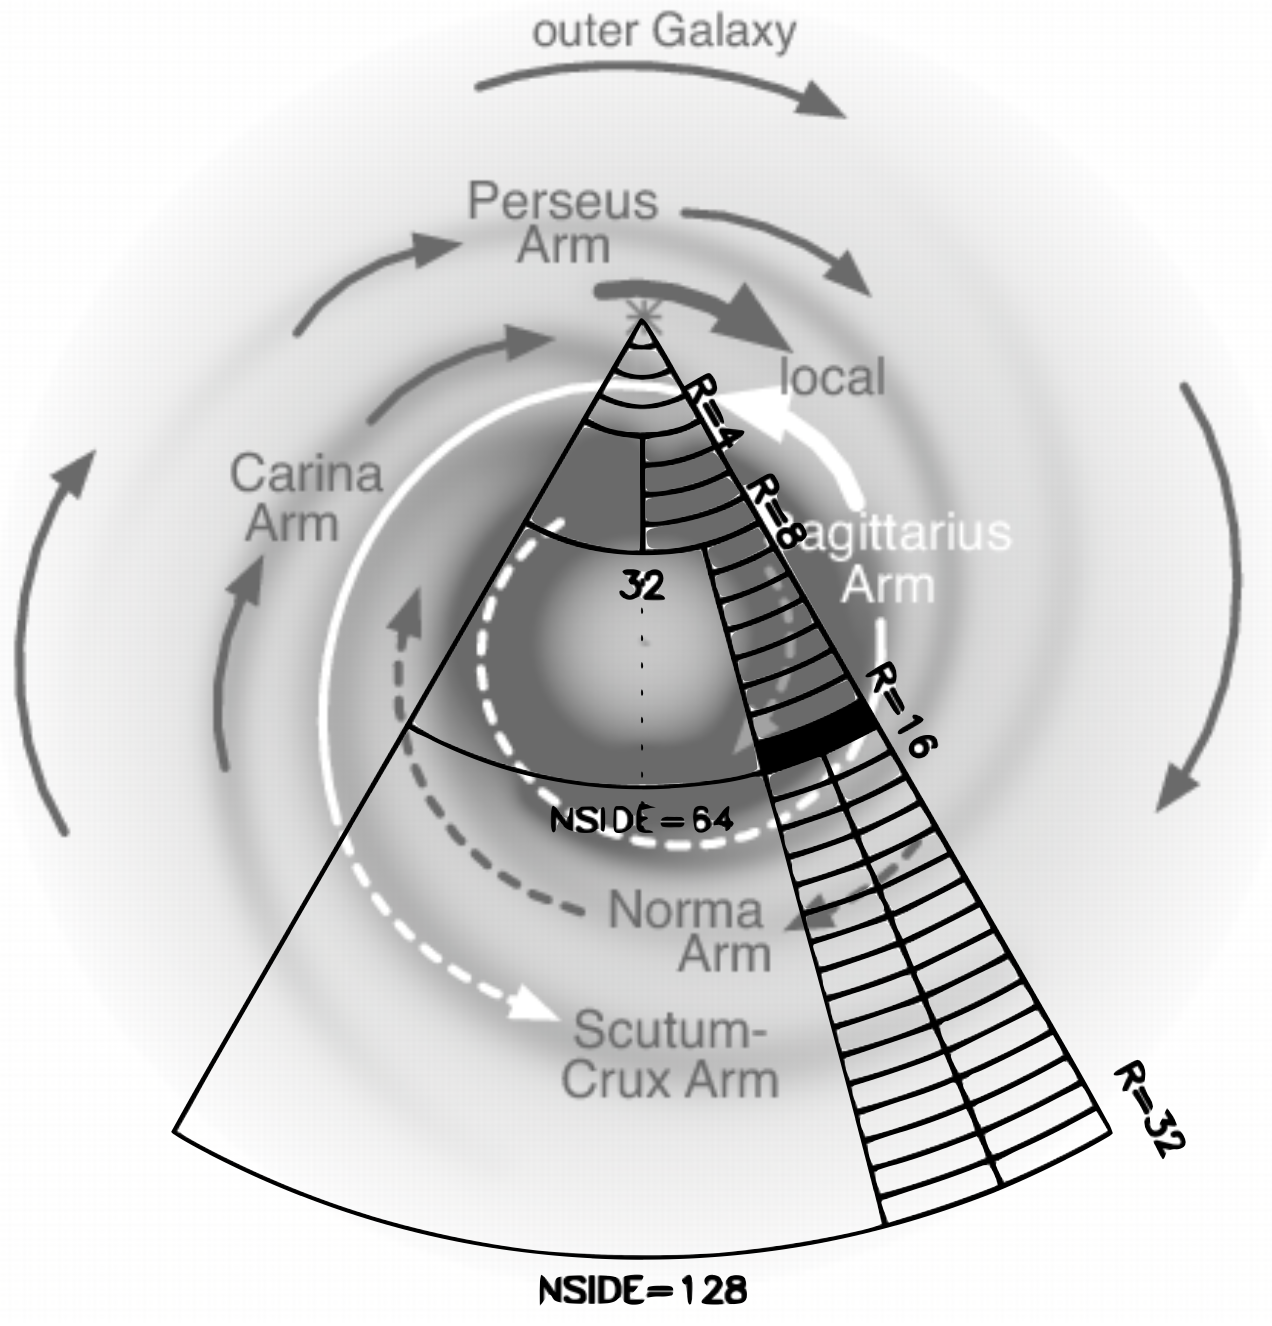
\includegraphics[width=0.45\textwidth]{cartoon.png} & 
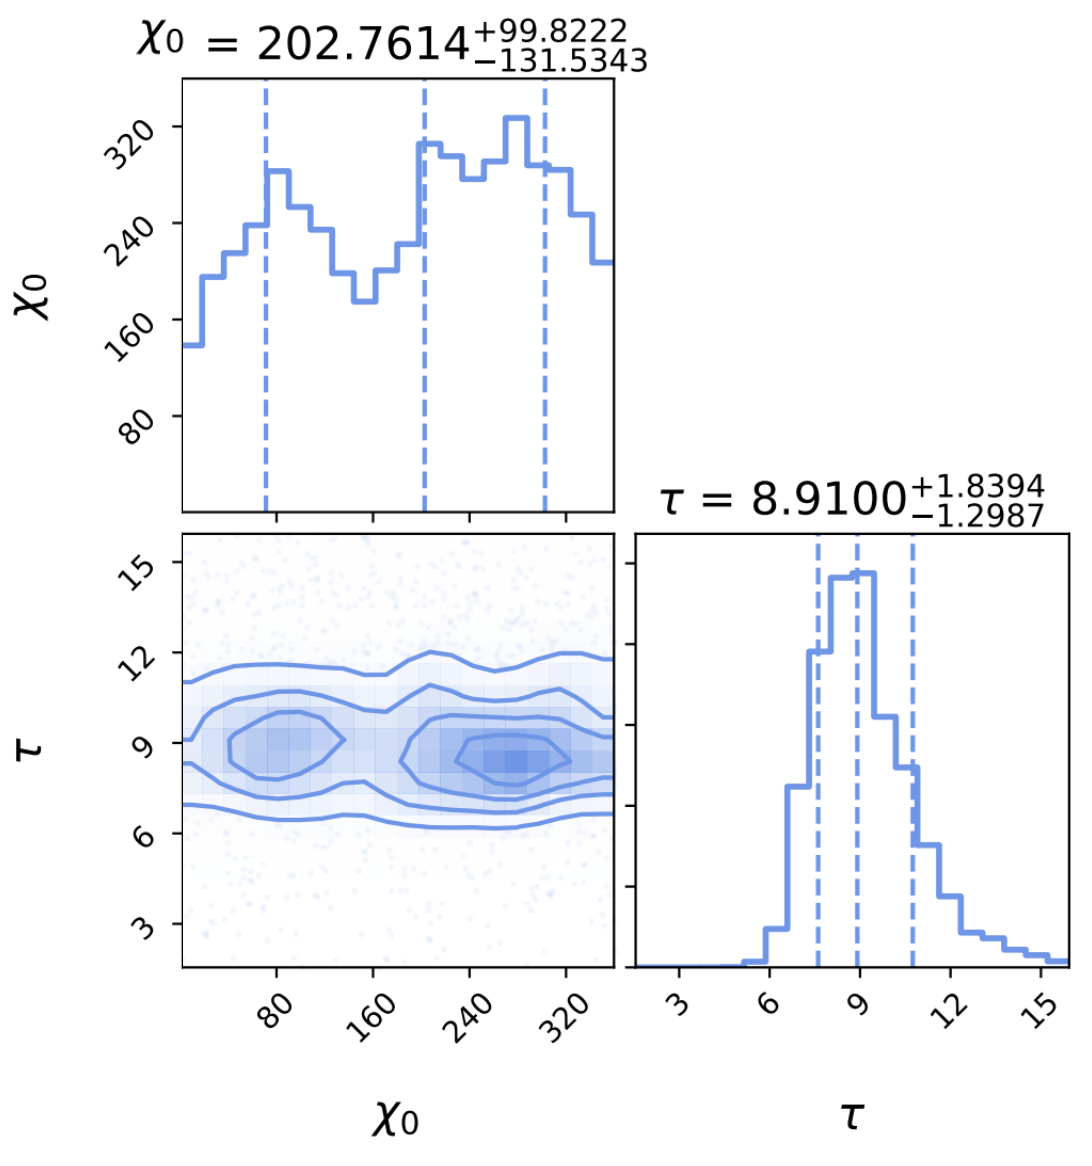
\includegraphics[width=0.5\textwidth]{cartoonL.png} \\
\end{array}$
\caption{
{\bf Left:} cartoon of how the \hammurabi\ code integrates through a galaxy simulation with a HEALPix-based grid that refines with distance. (Galaxy model from \citet{vaneck}. Grid courtesy X. Sun.)
{\bf Right:} example of part of the likelihood space mapped out in
\citet{steininger:2018} using the \imagineSW\ infrastructure. This
subset of the results shows $\chi_0$, the angle defining the tilt of
the field relative to the disc, and $\tau$, the strength of the random
component.  See text.
\label{fig:cartoon}
}
\end{figure}

%The \hammurabi\ integrator has also been integrated with the Galprop code of \cite{galprop} that connects the emitted synchrotron emission with the propagation of the cosmic rays. This was used in, e.g., \citet{orlando:2013} as well as the PIPXLII analysis. The new \hammurabix\ is being integrated with a different method of propagating cosmic rays developed by collaborator J. Wang that will provide a complementary view. 


\subsubsection*{Methods: cosmic ray propagation}

Most previous studies of synchrotron emission treated the GCRP independently of the GMF.  A self-consistent approach was demonstrated in \cite{jaffe:2011}, but more physically realistic GCRP codes are becoming available.  

There are several publicly available numeric GCRP packages with fast partial-differential-equation (PDE) solvers:  GALPROP \footnote{https://galprop.stanford.edu} and DRAGON \footnote{https://github.com/cosmicrays}.
GALPROP was developed with a FORTRAN solver and now has a C++ front-end, while DRAGON uses the same kernel from GALPROP but its front-end includes anisotropic diffusion and a pre-defined inhomogeneous grid that can focus the resolution more efficiently on the more interesting spatial regions such as the inner galaxy.
Both packages use the finite difference method in solving the CR transport equation with a built-in cross-section calculator to handle interactions and decays of various particle species.
Given a GMF realization and a CRL source description, we can run either DRAGON or GALPROP and find the steady-state distribution for CRLs.
The \hammurabi\ code can then take the phase-space distribution of propagated CRLs to integrate the synchrotron emission into sky maps, where the GMF realization is the same in both the GCRP step and for the integration of observables.  

J. Wang and collaborators are developing a new GCRP framework CAFE based on the deal.II \footnote{https://www.dealii.org} library. 
This framework solves PDE with the finite-element method (FEM) with either a  continuous or discontinuous Galerkin approach in a phase-space domain of up to 6 dimensions.
CAFE, once completed, may be the most precise but also expensive option for simulating GCRP with adaptive mesh refinement.  For this project, however, we will use only part of its capability, focusing on CR leptons over a limited energy range corresponding to the observing frequencies of synchrotron emission.  

% \todo{[Don't think this level of detail is necessary.  I suggest the sentence above and removing this para.]} \sout{In our project we do not need the complete versions of the CR propagators. For mid- and high-latitude analysis, we are more interested in spatially local CRLs and spectral behaviour within a limited energy range (based on the observing frequencies for synchrotron emission).  We only need to implement the lepton-related mechanisms in GCRP, while other heavy particle species can be ignored.  Simulating a full 3 or 6 dimension phase-space distribution would be too demanding for our purposes.  As a trade off between computing cost and accuracy, we can run a Galactic-scale CR simulator with either spherical-symmetric or axial-symmetric assumptions.}

%\sout{CRs cannot be treated with plasma theory, which makes such studies different from the cold ISM fluid that interacts with the GMF through MHD in the Galactic disk. In the galactic halo, CR diffusion is determined by the GMF configuration. Meanwhile, its streaming instability can power GMF turbulence in the halo, which also includes GMF turbulence advected from Galactic disk. }
The spatial diffusion of Galactic CRs is mainly determined by the turbulent GMF configuration. 
At the same time, the CR streaming instability can power a specific (``slab Alfvenic'', \citealt{Lazarian2006}) mode in the GMF turbulence.
The feedback between the CRs and the turbulent GMF influences the CR distribution, which in turn affects the power spectrum of the synchrotron emission (Fig.\,\ref{fig:planck}).
Theoretical and simplified simulation work has been done recently by \cite{Blasi2012} and \cite{Evoli2018} suggesting that including the CR streaming instability in the ISM turbulence is not only more physical than analytic simulation assumptions, but also capable of making new observational predictions.  Such detailed numerical studies of this interactive mechanism can be done in CAFE but not in GALPROP or DRAGON, and may be important for both accurate characterization and simulation of the synchrotron emission as a CMB foreground. 

At a minimum package interfacing level, we can connect the simplified GCRP routine with \hammurabi\ in order to connect the GMF to the Galactic synchrotron emission.
Thus instead of using a parameterized CR distribution, the GCRP mechanism will be an integral part of the process of constraining the GMF distribution within the \imagine\ framework.  At the next level, we can study the observational implications of the CR-induced turbulent GMF in the Galactic halo, which will help us understand more of the Galactic structure and the power spectrum of the synchrotron foreground emission.


\subsubsection*{Methods:  statistics}

Once we have simulated sky maps, we will use them to define statistics that characterize some physical aspect of the inputs, i.e., the turbulence and/or supernova-like shells.  There are a variety of statistics studied in the literature as mentioned above, from the polarization gradients used to measure Mach numbers using synchrotron emission \citep{Burkhart:2012} to various polarization statistics applied to Planck dust emission data \citep{pipXX,pipXXXIII}.  We will test the ability of our simulations to reproduce the observed statistical properties and select those with the best discriminatory power for inclusion on the likelihood exploration (next section).  

These are not necessarily the most interesting statistical properties from the point of view of CMB foreground separation.  It's a slightly different question how to determine which simulations are more characteristic of the true CMB foregrounds in the ways that most impact the search for the B-modes.  This will have to be determined by plugging such simulations into component separation algorithms to test how well they work based on the residuals compared to the input CMB maps.  This is an interesting challenge in and of itself for future work and is beyond the scope of the current proposal, which is the first step to make that progress possible by providing better input maps.  


\subsubsection*{Methods:  likelihood exploration and \imagineSW\ }

With simulated sky maps based on GMF models (including any combination of large-scale models, MHD turbulence, and/or shell structures), we can then begin to compare the theory with the data. Because of the high dimensionality of the parameter space, a Bayesian sampler is best suited for this analysis, and the \imagine\ infrastructure was developed for precisely this purpose.  

\citet{steininger:2018} demonstrated that the \imagineSW\ framework can optimize a 3D model to full sky data while including the treatment of the galactic variance.  It was applied as a proof-of-concept to a simple test case of an axisymmetric spiral GMF for the large scales and a GRF for the small-scale turbulent component. A portion of the marginalized likelihood space from one of the tests is shown in Fig.\,\ref{fig:cartoon}.  The two parameters shown are the $\chi_0$, the field's tilt angle relative to the disc, and $\tau$, the random magnetic field strength.  This demonstrates its ability to map out both relatively simple (i.e. Gaussian) likelihood distributions (like $\tau$) as well as more complex (e.g, bimodal) likelihood spaces (like $\chi_0$, where there is a degeneracy in the defined angle). The 1D marginalized distributions are shown as well as the 2D covariance between the two parameters, which allows us to learn where there are degeneracies in the parameter space (which there aren't between these two parameters).

We will apply this more powerful infrastructure to assess the current state-of-the-art models. We have demonstrated working versions of all the tools and are ready to perform the first real challenge among the different models with all available data.

Our contribution to the IMAGINE infrastructure will also include a quantification of the non-Gaussian statistics discussed in the previous section and their relationship to certain physical parameters.  For example, we may be able to probe the sonic Mach number of the turbulence by constructing a likelihood based on the polarization gradient measured with the input data.  


\subsection*{Work and management plan}


\subsubsection*{Plan:  team}

\begin{itemize}
\item PI T. R Jaffe (0.08 FTE/yr): Dr. Jaffe is one of the pioneers of
  this large-scale magnetic field analysis, from the
  first paper that performed a quantitative exploration of the
  likelihood space of a GMF model \citep{jaffe10} to having lead the \planck\ working group on large-scale field modeling and the PIPXLII paper. TJ is also: the responsible
  developer of the current \hammurabi\ software; a co-developer of the
  new \hammurabix\ software; a co-PI of the \imagine\ project. TJ is
  also a scientist with professional experience providing both software and high-level data
  products to the community.

\item Jiaxin Wang (1.0 FTE/yr): J. Wang is the primary developer of the CAFE CR propagation simulator and of \hammurabix, the new and improved integrator code, as well as a contributor to \imagineSW, and a researcher studying cosmic ray propagation in magnetic fields.  JW will perform the bulk of the work in this proposal in collaboration with TJ.  


\end{itemize}

This project will use the framework developed by the
\imagineC\, of which Dr. Jaffe is a co-PI. The tools are publicly
available, but the advantage of coordinating with the consortium is
regular contact with and input from experts in a variety of related
fields. In particular, we will work with the following collaborators:

\begin{itemize}
\item A. Shukurov and Graeme Sarson (University of Newcastle) will 
  provide MHD simulation cubes such as shown in Fig.~\ref{fig:mhd} and
  help with developing statistical and topological tools to analyze
  the 2D maps we generate.

\item T. En{\ss}lin (MPA, Munich) will provide expertise
  in the \imagineSW\ infrastructure and Bayesian methods in general;

\item F. Boulanger (ENS, Paris) is the lead of the
  MISTIC  project producing a large fraction of the new polarized dust results
  for the Planck Collaboration, including statistical tools we will apply to both data and simulated maps generated from MHD simulations; his group will provide MHD simulations such as those as used in \citet{pipXX}.  \end{itemize}



\subsubsection*{Plan:  timeline}\label{sec:outline}

For this project, we request funding for three years and support for
a post-doctoral researcher to perform the analysis using
and extending existing tools. 

\begin{itemize}

\item 0-6 months: (TJ+JW) make necessary modifications to the \hammurabi\ code to:   build an interface between to the CAFE, GALPROP, and DRAGON CR propagation codes;  improve the interface between \imagineSW\ and \hammurabi;  apply optimisation and parallelism to the full numerical pipeline. 
Each building block has to be strictly tested, profiled and optimised.

\item 6 to 18 months: (JW+TJ) implement the \imagineSW\
  infrastructure:   

\begin{itemize}


\item We will need to determine how many parameters can be
  optimized in a reasonable time-frame for each model.  This remains
  TBD with the new code and will involve testing on the computational
  platform for what is feasible. It is easy to calculate how long a
  given \hammurabi\ run will take. It is much harder to quantify how
  many {\it times} it will need to be run, as it is a function of the
  number of samples necessary for the Markov Chain to converge, which depends
  both on the algorithm used and the shape and size of the likelihood
  space being mapped out. One of the goals is to determine how large and complex a likelihood space can feasibly and uniquely be mapped out with the available data. We have flexibility in defining the scope of
  the analysis to fit the system constraints, so we will do the deepest analysis possible on the resources available, and
  it is guaranteed to be both new and interesting, precisely because
  nobody has done anything comparable before.

\item For each model, we will run the optimization with \imagineSW\ and all
  available data, including diffuse polarized synchrotron and dust emission as well as 
  Faraday RM data from
  \citet{oppermann:2012b}. \citealt{jaffe10} demonstrates why the
  RM observables are crucial.  For each model, we will quantify the Bayesian evidence that
  contains the real information about how much we have learned about
  the GMF from a given model fit. 


\item We will quantify the differences in the resulting GMF when the optimization is run with a consistent pipeline (where the GCRP is simulated based on the input GMF) or an inconsistent one (where CR electron/positron distribution is given independent from GMF).  

\item We can then test the impact of each morphological feature, such
  as the x-shaped field or individual spiral arm field reversals, and
  quantify whether its addition is justified by its effect on the
  improved fit to the data. We will also update the \hammurabix\ software encoding
  these models to construct a more generic parametrization and combinations of features. We will then be well prepared for the next step, 
  to fit models that include all 
  of the relevant morphological options, e.g., the Gaussian-profiled
  spiral arms of the Jaffe13 model added to the x-shaped halo field of
  JF12.

\end{itemize}

This part of the project will likely lead to at least two publications:  one will present the results of the Bayesian model comparison of the models in the literature; and a second paper will explore how we can select the most important features of these models and combine them in a more generic model parametrization. 
 
\item 18 - 36 months: analysis of the MHD turbulence simulation
  cubes. 

\begin{itemize}
\item (JW) We will then use \hammurabi\ to generate 2D integrated sky maps
  from the MHD cubes. The mid- to high-latitude sky requires only a
  single MHD cube with the observer at the center. We will also try to
  simulate the Galactic plane by modifying the integrator to tile the
  plane with cubes. With a small number of cubes that we can 
  randomly place and rotate, we can simulate a Galactic disc with different
  properties and see how the simulated observation beam affects the 
  integration through the long lines of sight.

\item (JW) We will also insert MHD simulations of the GMF turbulence into the cosmic-ray propagation simulator to observe the influence of the turbulence on the resulting CR electron/positron distribution.  In particular, the CR feedback into the Galaxy halo can be studied by using these simulated MHD cubes as a background source of  turbulence from Galactic disk. 

\item (JW+TJ) From the 2D maps we produce, we will define statistical characterizations that can be compared to those of the data {\it and} related back to the physical MHD parameters. For example, we can start with the phase coherence index of \citealt{burkhart:2016} that has been demonstrated to probe the MHD properties (e.g., Mach number). Collaborator F. Boulanger's group is also working with ``wavelet scattering transform'' that we will test as well.  We will also apply traditional CMB tools such as the bispectrum and Minkowski functionals etc., which in addition to being useful in the cosmological context will also help us to characterize the non-Gaussian fluctuations of the polarized foregrounds.

\item (JW+TJ) With these statistics applied to both the simulations and the data for the first time over the full sky, we will learn about the turbulent ISM in the local neighborhood. By comparing the observables from the different sets of MHD simulations and CR propagators, we will learn about the expected correlations between the dust and synchrotron emission in the different environments.  

\end{itemize}

This part of the project would produce at least one publication describing how we generate full sky maps from MHD simulations and what we learn from them about the statistical properties of the turbulence.  It should also produce a likelihood module for IMAGINE that quantifies whether the given data has the measurable statistics of certain MHD models.  (This module would be contributed to the publicly available IMAGINE repository.)  


\item (JW+TJ) Finally, we will publish our full sky maps % to the LAMBDA archive
  as a resource for the CMB community. This is very straightforward,
  as the community standard is FITS files in a HEALPix format, which
  is precisely what \hammurabi\ is designed to produce. 

\end{itemize}


\subsubsection*{Plan:  computation resources}

The High Performance Computing Center at the University of Maryland has several resources available such as the Deepthought cluster to which the Astronomy department has access.  The first part of this project requires some ~500 kCPU\,h of time on such a cluster to explore the likelihood space of the several models we wish to compare (as outlined above).  The test project in Steininger et al. (2018) used roughly 400 kCPU\,h of time on a similar computational facility. The software is already tested (and the speed improved since the Steininger et al. 2018 results were computed), so the proposed project is more ambitious, and we estimate we will need at least as much CPU time over the three year project. Note that this is the sort of project that will, by design, expand to fill the available computational resources, since when it comes to the resolution that we can achieve and the size of the parameter space, more is always better. This means that we are flexible and can adjust the parameter space probed as needed, and the results will still be unprecedented and instructive, since nothing of the kind has been done before.

We also request \$6k for a desktop machine for the postdoc. This machine will have to be powerful enough to run instances of the \imagineSW\ framework for local testing.  We will purchase a Linux or Mac desktop with sufficient resources, e.g., an iMac Pro with 8 cores, 64\,GB of RAM, and 1\,TB of disk space, along with an external backup drive.

Note that the second part of the project does not require large amounts of CPU time and could be performed on a high-end desktop machine or one of several linux machines available to us at UMD.  



\subsubsection*{Plan:  travel}

An important aspect of this project is collaboration with members of the \imagineC.  We will need to meet with A. Shukurov and G. Sarson to work with the MHD cubes and to interpret results from the 2D integrated sky maps. We will visit collaborator F. Boulanger, whose group is using a similar approach with a different set of MHD simulations focused on the dust emission, work that will be very useful to compare with this complementary project.  We will also attend semi-regular \imagineC\ meetings.  The proposed budget supports sufficient travel funds to meet face to face with our international collaborators as well as potential US-based collaborators and to travel to conferences to present results.  We anticipate one international and two domestic trips per participant per year.


\section*{Broader impacts}

Because of the ubiquity of magnetic fields in the Universe and their effect on the observables from many astrophysical contexts, this project will impact a variety of fields, from the understanding of our own Galaxy's dynamics and evolution to the origin of the Universe.  CMB scientists often simulate foregrounds using simple axisymmetric spiral models that do not capture more than the $0^\mathrm{th}$ order morphology of the magnetic field. At the other extreme, high energy astro-particle physicists studying cosmic rays often take the JF12 model at face value without taking into account its complexity and the likelihood of its having been over-fitted. Though the PIPXLII paper provided an analysis of the issues for all of these models, it elucidated problems that we were not yet able to solve. We now have the tools to provide to the community a set of large-scale magnetic field models that have been correctly optimized and statistically characterized.  Our understanding of how to create and maintain a magnetic field in a galaxy is currently quite limited but would be significantly advanced if we could measure it reliably in our own Milky Way.  Cosmic rays in the Galaxy cannot be studied without an understanding of the magnetic fields that are not only thought to be key to their acceleration but also to their propagation and equilibrium distribution.  The widespread use of the JF12 model in the ultra-high energy cosmic ray (UHECR) community is a sign of how much such a model is needed to understand the sources of these most energetic particles, since their deflection in the Galactic magnetic field confuses their extragalactic origin point.  For all of these topics, the first part of this project will provide the crucial quantitative model comparison that has been lacking.  

The comparison of simulated emission from MHD simulations with data have so far been performed in simple flat-sky approximations by integrating parallel to an edge of the simulation cube, which does not take into account the observational geometrical effects that are important for large angular scales and full-sky studies. We will be able to characterize how important these effects are in a given context, from the radio regime where Faraday effects dominate to the microwave and submm bands where they are negligible and instead the dust signal is more important, the synchrotron still significant, and the possible correlations between them not yet understood.  

CMB scientists also currently lack the tools to simulate realistic turbulence, but this comes naturally out of the second part of the project we define above. By combining the \hammurabi\ integrator with MHD simulations, we will produce sky maps that will be useful in a variety of contexts. In particular, planning for CMB S-4, the next-generation CMB observatory, aiming to detect primordial gravitational waves through their signature in the polarized CMB requires a far more detailed understanding of the turbulent foregrounds. The non-Gaussian nature of the Galactic signal, the possible correlations between synchrotron and dust emission, and the effect of the foregrounds on the systematics must be simulated more accurately than has yet been done in order to design the spectral and spatial coverage and resolution required to reach the interesting inflationary scales. This project will not solve the entire field but as a first step would provide MHD-based full-sky maps of these foregrounds that could be inputs to CMB end-to-end simulation pipelines and component separation challenges. 


\newpage
\bibliographystyle{abbrvnat}
\bibliography{science,jwangs}


\end{document}
